% todo: q5, q2.1
\documentclass[11pt,onecolumn,letterpaper]{article}
\usepackage{amsmath,amssymb,amsthm,graphicx,xspace,multirow,tikz}
\usetikzlibrary{arrows,automata,shapes}
\usepackage[titlenotnumbered,noend,noline]{algorithm2e}
\usepackage{listings}
\usepackage[compact]{titlesec}
\usepackage{XCharter}
\usepackage[T1]{fontenc}
\usepackage[scaled]{beramono}
\usepackage{multicol}

\tikzstyle{block} = [rectangle, draw, fill=blue!20, 
    text width=5em, text centered, rounded corners, minimum height=2em]
\tikzstyle{bt} = [rectangle, draw, fill=blue!20, 
    text width=4em, text centered, rounded corners, minimum height=2em]
\setlength{\evensidemargin}{-0.1in} \setlength{\oddsidemargin}{-0.1in}
\setlength{\textwidth}{6.5in} \setlength{\textheight}{9.0in}
\setlength{\topmargin}{-0.5in}
\setlength{\parindent}{0in}
\setlength{\parskip}{0.125in}

\newcounter{qNum}
\setcounter{qNum}{1}
%\newcommand{\q}[1]{\vspace*{0.10in} \noindent
%\arabic{qNum}.~(#1)\stepcounter{qNum}}
\newcommand{\q}[1]{%\vspace*{0.10in} \noindent
\textbf{(#1)}\stepcounter{qNum}}

\newcommand*\circled[1]{\tikz[baseline=(char.base)]{
    \node[shape=circle,draw,inner sep=2pt] (char) {#1};}}
    
\lstset{basicstyle=\footnotesize\ttfamily,breaklines=true}

\newcommand{\solpara}{\vspace*{0.0625in}\noindent\textbf{Solution}\hspace*{0.25in}}

\title{SE 465 W19 Midterm Solutions}
\author{Patrick Lam}

\begin{document}
\vspace{-12em}

\maketitle

\q{1}

Lots of changes are possible. I thought the obvious ones are changing
something in the {\tt if} condition but most of you changed one of the
{\tt +=} operators.

Say you changed {\tt vec == null} to {\tt vec != null}. You could use
the following test case:

\begin{lstlisting}
  @Test
  public void testAdd() {
    Location l1 = new Location(0.0, 4.65, 3.50, W);
    Location l2 = new Location(1.0, 2.0, 3.0, W2);
    l1 = l1.add(l2);
  }
\end{lstlisting}

Best practice if you were actually writing test code would be to
assert on the values in {\tt l1} after {\tt add}. On the other hand,
best practice for writing an exam is to keep the test case as small as
possible. I didn't say that you had to assert. If you do, that's great
(and the exams that I looked at all did). In my case, the actual and
expected behaviours for the original are successful executions with no
output. The actual output for the mutant would be a {\tt
  NullPointerException}. (You don't actually need expected output for
the mutant).

\newpage
\q{2}

Let's number the lines.

\begin{lstlisting}[language=Java,numbers=left]
    public int nextInt(int n) {
        if (n<=0)
            throw new IllegalArgumentException("n must be positive");

        if ((n & -n) == n)  // i.e., n is a power of 2
            return (int)((n * (long)next(31)) >> 31);

        int bits, val;
        do {
            bits = next(31);
            val = bits % n;
        } while(bits - val + (n-1) < 0);
        return val;
    }
\end{lstlisting}

\begin{center}
\begin{tikzpicture}[->,>=stealth',shorten >=1pt,auto,node distance=1.5cm,
                    semithick,initial text=]

  \node[initial,bt]   (1)                     {(L2)};
  \node[bt]           (2) [below right of=1,yshift=-1em]        {(L3)};
  \node[bt]           (3) [below of=1,yshift=-2.5em] {(L5)};
  \node[bt]           (4) [below right of=3,yshift=-1em] {(L6)};
  \node[bt]           (5) [below of=3,yshift=-2.5em] {(L8--9)};
  \node[bt,text width=6em]           (6) [below of=5] {(L10--11)};
  \node[bt,accepting]           (7) [below of=6] {(L13)};

  \path (1) edge node[yshift=-.5em] {T} (2)
  (2) edge node {} (3)
  (1) edge node[left] {F} (3)
  (3) edge node[yshift=-.5em] {T} (4)
  (4) edge node {} (5)
  (3) edge node[left] {F} (5)

  (5) edge node {} (6)
  (6) edge node {} (7)
  (6) edge [loop left] node {{\tt bits - val + (n-1) < 0}} (6)
        %% (3) edge node[left] {F} (4)
        %%     edge [bend left] node {T} (7)
        %% (4) edge node {} (5)
        %% (5) edge node {} (6)
        %% (6.west) edge [bend left=45] node {} (3.west)
            ;
\end{tikzpicture}
\end{center}

EDIT 2019-03-22: oops, there is no edge from L3 to L5. -PL

I don't actually care about little details like indicating the start
and end nodes. The general structure is sufficient for full marks. You can
omit lines 8--9 if you want. I just wanted to have an extra node for the entry
to the {\tt do} loop.

Statement coverage: Reachability of lines 1--5 depend on the input $n$.
Because it's a do-while loop, the body of the loop is also going to be
always executed as soon as line 6 is reached. And then line 10 is also
unconditionally executed as soon as line 6. So there are in fact
no difficulties in achieving 100\% statement coverage as long
as you pick the appropriate $n$.

Any terminating execution is going to get out of the loop, and it is
reasonable to assume that this function terminates since I said it
comes from the library. I guess you don't know for a fact that {\tt
  nextInt} terminates, so you should discuss potential issues with
termination.  Saying the assumption above is fine. Saying you don't
know is fine. Not saying the assumption but relying on it is 4/5.

To achieve 100\% statement coverage, you need $n$ strictly positive
(to reach line 3) and negative (line 2), and then you need {\texttt (n
  \& -n) == n} (you can believe the comment and provide $n$ a power of
$2$, $4$ for instance) and $n$ not a power of $2$, say 5.

Someone pointed out that setting $n=1$ ensures termination (you always get 0).
I didn't expect students to deduce that.

Marks breakdown: 3 points for saying that 100\% statement coverage
is achievable by choosing $n$, 2 points for finding the $n$.

Branch coverage is a bit harder. The {\tt if} statements are no harder. You need to make sure you go
around the loop once as well as out of the loop. The crux is making sure that the execution
goes around the loop, i.e. {\tt bits - val + (n - 1) < 0}. You don't know what {\tt next} is going to return,
but you can say that you set {\tt Random}'s state such that {\tt next(31)} returns something smaller than
{\tt val - (n-1)}. 

Same breakdown: 3 points for discussing the conditions, 2 points for specifically
saying how to achieve branch coverage.

\q{3}
Correct input: The easiest possible thing is to change one of the integers to a
different integer.

Incorrect input: Change the URL; or, in the request, modify or delete one of the field names.

I chose the number 4 so that you would have to provide at least one of the requests
that has a payload. The path of least resistance is to generate the three non-payload
requests with randomly-generated data and, say, POSTing {\tt /api/users}.

Pseudocode:
\begin{verbatim}
  choose a random number between 1 and 4
  case 1: generate request "GET /api/users"
  case 2: generate request "GET /api/users/"+random int
  case 3: generate request "DELETE /api/users/"+random int
  case 4: generate request "POST /api/users" 
             with payload {"name": random string, "job": random string}.
\end{verbatim}

You could also write down a context-free grammar but then you have to write
pseudocode for generating a string from the grammar, which is a lot of work.
It's OK if you say how to create string from parser, 4/6 if you just give the grammar.

Any reasonable modification of the pseudocode is OK. For instance you could
modify the request string, or change ``random int'' to ``random string'', or
change the field names.

\newpage
\q{4} It was in your interest to write as simple an FSM as you could
get away with. I didn't actually expect everything to be in the FSM,
and it was OK to abstract things away. I guess I could have been a bit more clear.

In my opinion, the best solution (but not the only one that gets full marks)
includes two subparts. One of the subparts is for register/login/logout.
Once logged in, then you can do all of the {\tt users} operations. It would
be fine to have only one of the subparts, and probably better for answering the exam.

\begin{center}
\begin{tikzpicture}[->,>=stealth',shorten >=1pt,auto,node distance=1.5cm,
                    semithick,initial text=]

  \node[initial,state]   (1)                     {1};
  \node[state]           (2) [right of=1,xshift=2em]        {2};
  \node[state]           (3) [right of=2,xshift=2em] {3};

  \path (1) edge node {register} (2)
  (2) edge[bend left] node {login} (3)
  (3) edge[bend left] node {logout} (2)
  ;

  \path[draw] (3) to [in=270,out=290,loop] node[auto,yshift=.5em,xshift=-.5em] {get} (3);
  \path[draw] (3) to [in=300,out=320,loop] node[auto,yshift=.5em] {getAll} (3);
  \path[draw] (3) to [in=330,out=350,loop] node[auto,yshift=.5em] {post} (3);
  \path[draw] (3) to [in=0,out=20,loop] node[auto] {put} (3);
  \path[draw] (3) to [in=30,out=50,loop] node[auto] {delete} (3);

\end{tikzpicture}
\end{center}


For the SRTC (2 points), each
node with a roundtrip needed to be represented in one of the test
requirements.  (While looking through the exams, I realized that the
SRTC definition does not require one roundtrip per node with a cycle,
i.e. multiple nodes can share the same cycle).  The test suite was
another 2 points, and then CRTC was another 2 points.

The safest way to answer SRTC here is the requirements $\{(2, 3, 2), (3, 2, 3), (3, 3)\}$
although you can definitely argue for smaller sets which contain at least
one cycle for each node, e.g. $\{2, 3, 2\}$ seems to meet the definition as I read
it today. CRTC adds all of the round trips starting at $3$. You should probably include
the $(3, 2, 3)$ cycle, because you can argue that it's different from the $(2,3,2)$ cycle.

Note that you have to satisfy the test requirements that you give. So
if you give a cycle for each node, then your test suite also has to
satisfy that cycle, e.g. if you say $(a, b, c, a), (b, c, a, b)$
(among others) then you need the cycles starting at both $a$ and $b$
in your test suite.  In that case, your test suite might miss going
around a cycle from the point of view of each node in the cycle, so
you would typically need to go around the cycle twice. But it's
actually OK to have test requirements that only include $(a, b, c,
a)$.

\q{5a}

Multiple acceptable answers, but exploratory testing is most useful
where human judgment is useful in identifying the correct
behaviour. UI/UX bugs are a good specific example and when I was
skimming answers, most of the good ones talked about UI bugs.  (The
lecture notes talk more about situations where exploratory testing is
useful, rather than about specific bugs you might catch).

\q{5b}
Fact 1: 55\% of statements were executed by test cases. Fact 2: These statements
did not throw uncaught exceptions.
One answer I saw was ``these statements are reachable''. That is correct so it
gets full marks. I was hoping for something more actionable, as in Fact 1 above.

\q{5c}
``Nothing'' is a correct answer. Also ``these statements are not reachable by your testcases''. Everyone I looked at got this.

\q{5d}
Looking for ``page objects''. Extra sentences that contained mis-facts would trigger deductions.

\q{5e}
I'd expect there to still be a failure. I thought that the fault would now be at the previous
write to the same state. Answers saying that the fault was at the next access to that
state are OK too.



%% \begin{lstlisting}[language=C]
%% void process( char* buffer ); /* Implementation not shown */

%% int main( int argc, char** argv ) {
%%   char* buffer1 = malloc( MAX_SIZE * sizeof( char ));
%%   char* buffer2 = malloc( MAX_SIZE * sizeof( char ));
  
%%   int fd = open( argv[1], O_RDONLY );
%%   memset( buffer1, 0, MAX_SIZE * sizeof( char ));
%%   read( fd, buffer1, MAX_SIZE );
%%   close( fd );
  
%%   for ( int i = 2; i < argc; i++ ) {
%%     int nextFD = open( argv[i], O_RDONLY  );
    
%%     aiocb cb;
%%     memset( &cb, 0, sizeof( aiocb ));
    
%%     cb.aio_nbytes = MAX_SIZE;
%%     cb.aio_fildes = nextFD;
%%     cb.aio_offset = 0;
%%     if ( i % 2 == 0 ) {
%%       memset( buffer2, 0, MAX_SIZE * sizeof( char ));
%%       cb.aio_buf = buffer2;
%%     } else {
%%       memset( buffer1, 0, MAX_SIZE * sizeof( char ));
%%       cb.aio_buf = buffer1;
%%     }
%%     aio_read( &cb );
 
%%     if ( i % 2 == 0 ) {
%%       process( buffer1 );
%%     } else {
%%       process( buffer2 );
%%     }
    
%%     while( aio_error( &cb ) == EINPROGRESS ) {
%%       sleep( 1 );
%%     }
%%     close( nextFD );
%%   }
%%   free( buffer1 );
%%   free( buffer2 );

%%   return 0;
%% }
%% \end{lstlisting}



\end{document}
